\section{\methodname}
\label{sec:method}

\begin{figure}[t]
	\centering
	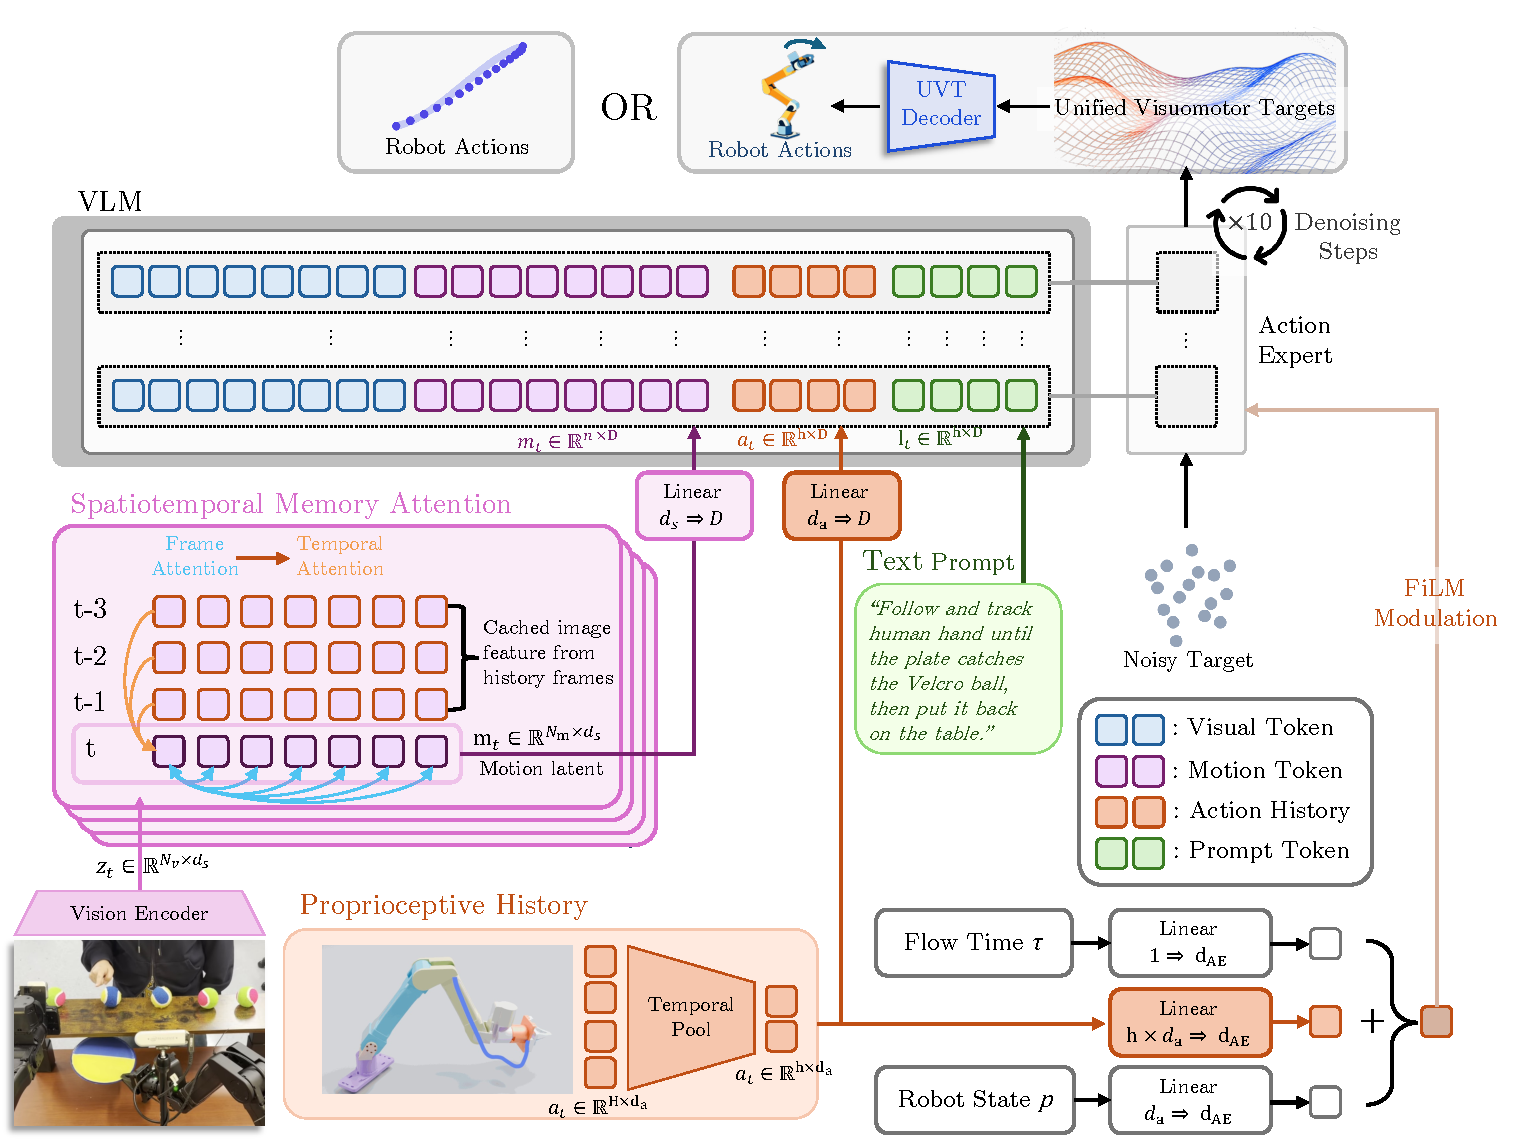
\includegraphics[width=0.95\columnwidth]{2026-corl-unveil-template/figures/tempo_main.pdf}
	\vspace{-0.6em}
	\caption{\textbf{\ours\ architecture.} \ours\ augments a pretrained VLM-based policy with two temporal inputs. \TEMPOMOT\ cross-attends the current frame's patch features $\mathbf{f}_t$ against a streaming cache $\mathcal{F}_t$ of features from the preceding $W-1$ frames, producing a motion code $\mathbf{m}_t$ that encodes scene dynamics. \TEMPOACT\ mean pools the robot's recent proprioceptive command history into $K$ fixed-size buckets, yielding a compact summary $\mathbf{c}_t$. Both signals attach to the pretrained backbone with near-zero overhead: $\mathbf{m}_t$ and $\mathbf{c}_t$ are projected to the VLM's token dimension and appended to its prefix, and $\mathbf{c}_t$ additionally conditions the action expert via an AdaRMS residual.}
	\label{fig:method}
\end{figure}
% we can add an optional module uvt 

\ours\ supplies the two temporal signals that \cref{sec:diagnosis} identifies as missing: \TEMPOMOT, a motion encoder that summarizes recent scene dynamics, and \TEMPOACT, a compact proprioceptive history. Both attach to a pretrained VLA with near-zero overhead (\figref{fig:method}).


\vspace{-0.3em}
\subsection{\TEMPOMOT: Captures Object and Scene Dynamics}
\TEMPOMOT\ summarizes recent visual dynamics by cross-attending the current frame against a rolling cache of past frames (\figref{fig:method}). Let $\mathbf{f}_\tau$ denote the patch features of observation $o_\tau$, extracted by $\phi$'s per-frame encoder. Over a streaming window of length $W$, we maintain a cache $\mathcal{F}_t = \{\mathbf{f}_\tau\}_{\tau=t-W+1}^{t-1}$ of features from the preceding $W-1$ frames, populated incrementally so that each $\mathbf{f}_\tau$ is computed exactly once and reused on subsequent steps at no additional cost. The motion code is then
\begin{equation}
\label{eq:tempomot}
\mathbf{m}_t \;=\; \phi(o_{t-W+1:t}) \;=\; \operatorname{CrossAttn}\bigl(\mathbf{f}_t,\; \mathcal{F}_t\bigr),
\end{equation}
with the current-frame features $\mathbf{f}_t$ as queries and historical visual features as keys and values.

\begin{wraptable}{r}{0.42\columnwidth}
\centering
\vspace{-\baselineskip}
\small
\setlength{\tabcolsep}{4pt}
\begin{tabular}{lc}
\toprule
Motion encoder $\phi$ & Handover \\
\midrule
SAM~2.1-Tiny~\cite{sam2} (default) & \textbf{74\%} \\
Reducio~\cite{reducio}       & \textbf{76\%} \\
VidTwin~\cite{vidtwin}       & 60\% \\
VideoLaVIT~\cite{videolavit} & 52\% \\
\bottomrule
\end{tabular}
\caption{\textbf{Swapping the motion encoder $\phi$} keeps Bottle Handover success comfortably above the VLASH baseline ($38\%$).}
\label{tab:encoder_swap}
\end{wraptable}
We instantiate $\phi$ with a frozen pretrained video foundation model, used off-the-shelf without motion-specific fine-tuning; SAM~2.1-tiny~\cite{sam2} is our default. The choice is flexible: any video encoder whose features separate motion from appearance can serve as $\phi$. \figref{fig:ball_velocity_probe} shows that object velocity is linearly decodable from $\mathbf{m}_t$ computed from different video encoders, substantially outperforming a position-only baseline, across several encoder families, and \cref{tab:encoder_swap} confirms the same conclusion at the task level: swapping $\phi$ across four video foundation models keeps Bottle Handover success in the $52$–$76\%$ range, all well above the VLASH baseline. Reducio slightly exceeds our SAM default; we still adopt SAM~2.1-Tiny for the streaming speed required at real-time control rates (\tabref{tab:latency_comparison}).

\vspace{-0.3em}
\subsection{\TEMPOACT: Resolves State Aliasing}
Where \TEMPOMOT\ captures how the scene is moving, \TEMPOACT\ captures what the robot has been doing. A compact summary of recent proprioceptive history gives the temporal context for the robot policy to commit to the correct task phase. Without resolving state aliasing, the policy averages over multiple valid actions for the same observation, often producing indecisive behavior (e.g., pausing) or oscillating between conflicting actions, as seen in our baseline rollouts (\cref{fig:ambiguity}).

Raw proprioceptive history is long, high-frequency, and largely redundant, so we compact it into a fixed-size summary $\mathbf{c}_t$ (\TEMPOACT). Let the proprioceptive command at time $\tau$ be $q_\tau\in\mathbb{R}^{d_q}$. We consider the most recent $H$ commands preceding time $t$, partition them into $K$ contiguous temporal buckets $B_1,\ldots,B_K$ of equal length $L$ (so that $H=KL$), ordered from oldest to newest, and summarize each bucket by its mean:
\begin{equation}
\label{eq:joint-compaction}
\mathbf{c}_t=\bigl(\bar q^{(1)}_t,\dots,\bar q^{(K)}_t\bigr),\qquad
\bar q^{(k)}_t=\frac{1}{L}\sum_{\tau\in B_k} q_\tau\in\mathbb{R}^{d_q},\qquad
q_\tau:=0\ \text{for }\tau<\text{episode start}.
\end{equation}
% \vspace{-0.5em}

We use $K=10$ buckets, each averaging $L=30$ consecutive commands. Buckets that fall entirely before the episode start are marked with a pad flag. The resulting representation $\mathbf{c}_t\in\mathbb{R}^{K\times d_q}$ always contains $K$ tokens, regardless of how much history it summarizes. Extending the temporal horizon only changes the bucket length $L$, not the number of tokens. This simple, parameter-free aggregation preserves a coarse trend of robot's recent motion while adding negligible computational overhead.

\vspace{-0.3em}
\subsection{Plug-and-Play Temporal Integration}
We add the two signals to a pretrained VLA while keeping the pretrained backbone largely intact (\figref{fig:method}). We build on VLASH's asynchronous-inference pipeline~\cite{vlash} as the backbone, though our additions are agnostic to this choice. $\mathbf{m}_t$ is projected to the VLM's token dimension and appended to its prefix alongside the current multi-view observation and the language instruction. The action expert reads the resulting VLM prefix through the cross-attention layers. 

The $K$ bucket tokens of $\mathbf{c}_t$ are used in two ways. First, they are projected into VLM's prefix tokens dimension and appended to the VLM token stream, allowing the multimodal prefix to include the robot's recent proprioceptive history. Second, the same bucket sequence is flattened and passed through a conditioning MLP to produce an AdaRMS residual for the action expert, modulating the denoising process directly. 

Together, the two temporal signals provide complementary temporal contexts to the VLA.
The added conditioning path is zero-initialized, so the pretrained policy's behavior is preserved at the start of fine-tuning. Flow-matching loss is unchanged, and \ours\ adds only 2M~($0.08$\%) parameters.

\vspace{-0.3em}
\subsection{Real-Time Deployment via Parallel Encoding}
\begin{wraptable}{r}{0.40\columnwidth}
\centering
\vspace{-\baselineskip}
\small
\setlength{\tabcolsep}{4pt}
\begin{tabular}{lc}
\toprule
\textbf{Method} & \textbf{Median} \\
\midrule
VLASH~\cite{vlash}          & 33.8 ms \\
RTC~\cite{rtc}              & 127.7 ms \\
\ours~(Ours)                & 35.3 ms \\
\bottomrule
\end{tabular}
\caption{Inference latency comparison across methods.}
\label{tab:latency_comparison}
\end{wraptable}
\TEMPOMOT\ is encoded in a dedicated background thread, decoupled from the control loop: the motion encoder consumes camera frames at sensor rate ($\sim$11\,ms per frame on an NVIDIA RTX PRO 6000) and continuously updates the latest motion token, which the policy reads at each control step. The only overhead the policy pays is about 1.5\,ms for attending to the extra token (35.3\,ms vs.\ 33.8\,ms median forward time; \tabref{tab:latency_comparison}), versus approximately 128\,ms per chunk for the asynchronous baseline RTC~\cite{rtc}. Because $\phi$ operates over a fixed-size streaming window, its per-frame cost stays constant regardless of history length, so \ours\ adds motion awareness without impacting the policy's control rate.

%===============================================================================
